\begin{enumerate}[label=\thesection.\arabic*.,ref=\thesection.\theenumi]
\numberwithin{equation}{enumi} 
\item The open loop transfer function of a feedback control system is  
\begin{align}
G(s) = \frac{1}{s(1+2s)(1+s)} 
\label{ee18btech11016_gs}
\end{align}
%
Find the magnitude and phase of $\abs{G\brak{\j\omega}}$.
\\
\solution
\begin{align}
G\brak{\j\omega} &= \frac{1}{\j\omega(1+2\j\omega)(1+\j\omega)} 
\\
 &= \frac{1}{\j\omega(1+3\j\omega-2\omega^2)}=\frac{1}{\j\omega-3\omega^2-2\j\omega^3}
\\
 &= \frac{1}{-3\omega^2+\j\omega(1-2\omega^2)} 
\\
\implies \angle G\brak{\j\omega}&=- tan^{-1}\brak{\frac{\omega(1-2\omega^2)}{-3\omega^2}}
\label{ee18btech11016_gs_ang}
\end{align}
%
\item The frequency at which the phase of open-loop transfer function reaches -180$\degree$ or +180$\degree$ depending upon the range of tan inverse function) is defined to be the phase crossover frequency.  Find the phase crossover frequency for  \eqref{ee18btech11016_gs}.
\solution From \eqref{ee18btech11016_gs_ang}, at $\omega=\omega_{pc}$ 
\begin{align}
\omega(1-2\omega^2) = 0 
\\
\implies \omega_{pc} = \frac{1}{\sqrt{2}} 
\end{align}
\item The gain Margin is given by,
\begin{align}
GM = -20log_{10}\abs{G\brak{\j\omega_{pc}}} = 20log_{10}k_{g}
\end{align}
where 
\begin{align}
k_{g}=\frac{1}{\abs{G\brak{\j\omega_{pc}}}} 
\end{align}
%
Find the GM for \eqref{ee18btech11016_gs_ang}.
\\
\solution 
\begin{align}
\abs{G\brak{\j\omega_{pc}}} &= \frac{1}{\brak{\frac{3}{2}}}
\implies k_{g}&=\frac{1}{\abs{G\brak{\j\omega_{pc}}}} = \frac{3}{2}
\end{align}
i.e G.M = 3.5dB
\\

The greater the Gain Margin (GM), the greater the stability of the system. The gain margin refers to the amount of gain, which can be increased or decreased without making the system unstable. It is usually expressed as a magnitude in dB.
\item Obtain the GM from the Bode plot.
\solution The following code 
\begin{lstlisting}
codes/ee18btech11016.py
\end{lstlisting}
%
plots the amplitude and phase of \eqref{ee18btech11016_gs} in Fig. \label{fig:ee18btech11016}.
%
\begin{figure}[htp]
	\centering
	\includegraphics[width=\columnwidth]{./figs/ee18btech11016/fig.eps}
	\caption{}
	\label{fig:ee18btech11016}
\end{figure}
So,in the above figure, since $20log_{10}(G(\j\omega_{pc}))$ = -3.5dB at $\omega_{pc} = -180\degree$ so GM = +3.5dB. 
\item A positive GM indicates closed loop stability with unity feedback.  Verify this for \eqref{ee18btech11016_gs}.
\\
\solution 
The characteristic equation is 
\begin{align}
1+G(s)=0 
\implies 2s^3 + 3s^2 + s + 1 = 0 
\end{align}
Constructing the routh array
\begin{align}
\mydet{s^3\\s^2\\s}
\mydet{2 & 1 & 0 \\ 3 & 1 & 0 \\ (1/3) & 0 & 0}
\\
\mydet{s^3\\s^2\\s\\s^0}
\mydet{2 & 1 & 0 \\ 3 & 1 & 0 \\ (1/3) & 0 & 0 \\ 1 & 0 & 0}
\end{align}\\
%
There are no sign changes in the first column of the routh array. 
$\therefore$ the system is stable.
\\

\item Instead of unity feedback, consider a system with 
%
\begin{align}
H(s)=\frac{1}{s+1}
\end{align}
%
Compute the open loop gain margin for this system.
\\
\solution 

\begin{align}
\because G(s)H(s)=\frac{1}{s(1+2s)(s+1)^{2}},
\end{align}

Find the magnitude and phase of $\abs{G\brak{\j\omega}H\brak{\j\omega}}$
\begin{align}
G(j\omega)H(j\omega) = \frac{1}{(2\omega^4-4\omega^2) +j(\omega-5\omega^3)}
\end{align}
\begin{align}
=> \angle G(j\omega)H(j\omega) = -tan^{-1}(\frac{\omega-5\omega^3}{2\omega^4-4\omega^2})
\end{align}

Now , for $\omega$=$\omega_{pc}$ , the imaginary part of $G(j\omega)H(j\omega)$=0. i.e,
\begin{align}
\omega(1-5\omega^2)=0
=>\omega_{pc} = \frac{1}{\sqrt{5}}
\end{align}
\begin{align}
G.M = -20log_{10}|G(j\omega_{pc})H(j\omega_{pc})| = 20log_{10}k_{g}
\end{align}
where 
\begin{align}
k_{g}=\frac{1}{|G(j\omega_{pc})H(j\omega_{pc})|}
\end{align}
So, $k_{g}$ = $\frac{1}{\frac{1}{\frac{18}{25}}}$ = 18/25.
\\

And hence G.M=-2.853dB.i.e the gain margin is negative and hence we can say that the system is unstable.

\item Obtain the GM from the Bode plot.
\solution The following code 
\begin{lstlisting}
codes/ee18btech11016_2.py
\end{lstlisting}
plots the amplitude and phase of in Fig.
\begin{figure}[htp]
	\centering
	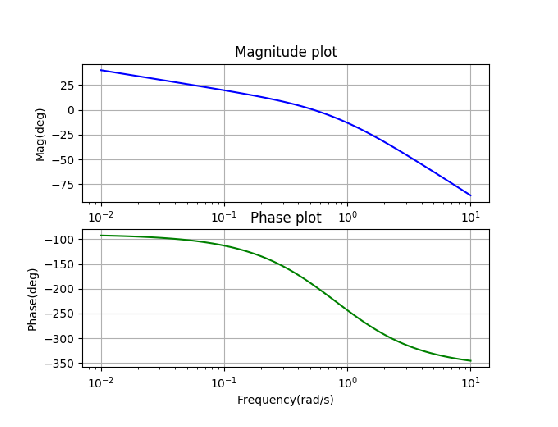
\includegraphics[width=\columnwidth]{./figs/ee18btech11016/fig2.eps}
	\caption{}
	\label{fig:ee18btech11016}
\end{figure}

\item 
Let's verify this using the RH array :
So,the closed loop transfer function is given by 
\begin{align}
T(s) = \frac{1}{1 + (s(1+2s)(1+s)^2)}
\end{align}

\begin{align}
=> D(s) = 1 + s(1+2s)(1+s)^2 = 2s^4+5s^3+4s^3+s+1
\end{align}
\\
So,the characteristics equation is given by D(s) = 0.i.e,
\begin{align}
=> 2s^4 + 5s^3 + 4s^3 + s + 1 = 0 
\end{align}
Constructing routh array for above equation of D(s),
\begin{align}
\mydet{s^4\\s^3\\s^2}
\mydet{2 & 4 & 1 \\ 5 & 1 & 0 \\ (18/5) & 1 & 0}
\end{align}

\begin{align}
\mydet{s^4\\s^3\\s^2\\s}
\mydet{2 & 1 & 0 \\ 3 & 1 & 0 \\ (18/5) & 1 & 0 \\ (-7/18) & 0 & 0}
\end{align}

\begin{align}
\mydet{s^4\\s^3\\s^2\\s\\s^0}
\mydet{2 & 1 & 0 \\ 3 & 1 & 0 \\ (18/5) & 1 & 0 \\ (-7/18) & 0 & 0 \\ 1 & 0 & 0}
\end{align}

There are 2 sign changes in the first column of the routh array. So, 2 poles lie on right half of s-plane. 
\\
Therefore,the system is unstable.\\

Hence,we can say that from both Routh-hurwitz criterion and from the gain margin concept we are getting the same answers.
\end{enumerate}


